\documentclass[journal]{IEEEtran}
\usepackage[T1]{fontenc}
\usepackage{amsmath,amssymb}
\usepackage{graphicx}
\usepackage{booktabs}
\usepackage{array}
\usepackage{tabularx}
\usepackage{adjustbox}
\usepackage{placeins}
\usepackage[numbers,sort&compress]{natbib}
\usepackage{url}
\usepackage[hidelinks]{hyperref}
\usepackage{xr}  % labels and citations of the other document, under its prefix
\emergencystretch=2em  % long file names in \texttt

% Generated by paper/build_latex.py --ieee from PAPER.md and paper/ieee/front.md; edit those, not this file.

\externaldocument[S-]{supplement}  % Appendices A-J; compile main, supplement, main

\begin{document}

\title{Telling Night from a Failing Camera: Context-Gated Test-Time Adaptation for Maritime Detection}

\author{{\small\begin{tabular}[t]{@{}c@{}}
\normalsize Laksh Saroha\\
\textit{Department of Electronics and Communication Engineering}\\
\textit{Thapar Institute of Engineering and Technology}\\
Patiala, India\\
lsaroha\_be24@thapar.edu
\end{tabular}}
\hspace{2.5em}
{\small\begin{tabular}[t]{@{}c@{}}
\normalsize Sandeep Mandia\\
\textit{Department of Electronics and Communication Engineering}\\
\textit{Thapar Institute of Engineering and Technology}\\
Patiala, India\\
sandeep.mandia@thapar.edu
\end{tabular}}}

\markboth{}{Saroha and Mandia: Context-gated test-time adaptation}

\maketitle

\begin{abstract}
Visible cameras on surface vessels degrade in fog, low light, glare and noise, and so do their detectors. Re-estimating a detector's batch-normalization (BatchNorm) statistics at test time needs no labels, but on development, adapting every frame cost up to 0.023 average precision (AP) at night. The difficulty is deciding which frames to adapt: a dark visible frame may show a dark scene or a failing camera, and the visible image's health score flags every clean night frame. On the Pohang Canal dataset with simulated corruptions, we compare three pre-registered answers. Infrared-gated BatchNorm adaptation (IG-BN) adapts only when the visible frame looks abnormal and a healthy co-mounted thermal camera reports daylight; it needs no gradients or weight changes. IG-BN improved 5 of 60 development conditions and worsened none. On a held-out daylight run it raised ship AP under fog (+0.037), low light (+0.019), glare (+0.031, with a glare term) and sensor noise (+0.182). A clock gate using solar elevation instead was never worse than IG-BN on development and better in 13 conditions, all with a degraded thermal image. Shallow BN-mix, adapting the first 31 of 130 BatchNorm layers by each block's drift from training statistics, needs no day--night signal: it improved 24 development and 3 held-out conditions and worsened none. We match each answer to the sensors available. On held-out daylight, and on average on unseen night frames, adapting every frame did best, so gating is the safe choice, not a proven necessity. All thirteen held-out scorings are logged.
\end{abstract}

\begin{IEEEkeywords}
Batch normalization, infrared imaging, maritime object detection, sensor fusion, test-time adaptation, thermal imaging, unmanned surface vehicles, visible--infrared detection
\end{IEEEkeywords}

\section{Introduction}\label{sec:1}
Maritime perception for autonomous and crewed surface vessels increasingly pairs a visible camera with a long-wave infrared (thermal) camera, on the assumption that the two fail in different conditions. A missed vessel or buoy is a collision risk, and fog, darkness, glare and sensor noise make misses more likely. Visible imagery degrades in fog, haze, glare, rain, darkness and sensor noise \cite{prasad2017video}. Thermal imagery sees through darkness and glare but fails at thermal crossover, when vessel and water reach the same temperature. Neither failure is signaled by the detector. A visible detector trained on clean frames meets a fogged or underexposed frame with activation statistics its BatchNorm layers were not fitted to, and returns fewer and worse boxes.

Test-time adaptation of normalization statistics is a low-cost repair. Replacing the BatchNorm statistics with those of a test batch \cite{li2017revisiting}, or mixing the two, which \citet{schneider2020improving} call BN-mix, needs no labels, no gradient computation and no weight changes, and it recovers much of the loss under common corruptions. The open problem is which frames to adapt. Adapting a frame that was never degraded moves a well-fitted detector away from its training statistics: in a pre-registered ablation on our development set, BN-mix applied to every frame gained on corrupted day frames but cost 0.0101 ship AP on clean day frames and 0.0195 on clean night frames (Section~\ref{sec:5.1}). On our held-out daylight run, adapting every frame gained about 0.02 on clean frames, and on unseen night frames it gained on average while losing on one of two stretches (Section~\ref{sec:5.3}), so the demonstrated harm of ungated adaptation is confined to development frames. Existing selective methods decide which samples to adapt from the model's own outputs or features (Section~\ref{sec:2}). A single visible camera faces an ambiguity that such signals do not resolve: a dark frame may show a dark scene, which the detector was trained on, or a degraded camera, which it was not. Our visible health score, fitted on clean day frames, flags all 1,032 clean night frames of our development set as unhealthy and none of the 1,200 clean day frames (Section~\ref{sec:4.1}).

The day--night signal has to come from outside the visible pixels, or the adaptation has to work without one. We compare three answers, each pre-registered (Section~\ref{sec:4}). The first takes its day--night signal from a co-mounted thermal camera. Infrared-gated BatchNorm adaptation (\mbox{IG-BN}) adapts the visible detector only when three conditions hold: the visible frame looks unhealthy, the thermal frame reads daylight, and the thermal frame is itself healthy (Fig.~\ref{fig:1}). A dark visible frame that the thermal camera places in daylight is treated as a degraded camera and adapted; one it places at night is left alone. The second, the clock gate, keeps the visible term and puts the sun's elevation, from time and position, in place of both thermal terms. The third needs no such signal: shallow BN-mix adapts only the shallowest BatchNorm layers, on every block, in proportion to how far the block's statistics have drifted from those of clean training data.

Our contributions are:

\begin{enumerate}
\item \textbf{The problem, measured.} Adapting a visible detector's BatchNorm statistics needs a decision about which frames to adapt, and on dark frames the visible camera cannot make it. Its health score flags every clean night frame; the feature-distribution gap of \citet{yoo2024what} activates on 90--100 percent of night frames; and in a pre-registered ablation, adapting the whole network without a day--night signal lost up to 0.0233 ship AP on development night frames, though not on average on unseen night frames (Sections~\ref{sec:4.1} and~\ref{sec:5.1}).
\item \textbf{Three answers under one pre-registered protocol, and when to use each.} \mbox{IG-BN}, gated by the thermal camera, is the most tested. Six of its seven forms passed development on 60 cells with no cell worse; the seventh (\mbox{IG-BN-stale}) failed and was dropped. On a held-out daylight run none of the six was worse than its baseline on any cell, with gains under fog (+0.0370 ship AP), low light (+0.0186), glare with the glare term (+0.0309) and, in a first test, sensor noise (+0.1823). We found no prior test-time adaptation for visible--infrared detection in which the thermal camera decides, without gradients, when to adapt the visible detector (Section~\ref{sec:2}). The clock gate was never worse than \mbox{IG-BN} on development and better on 13 cells, all with a degraded thermal stream. Shallow BN-mix, with no day--night signal, was better on 24 development cells and three held-out cells and worse on none, with night changes within noise on development and on unseen night frames (Section~\ref{sec:5}). We turn them into a choice by the signals available (Section~\ref{sec:7}).
\item \textbf{Negative results from the same system.} We reached these designs by elimination. Predicted box uncertainty is informative about which boxes are right but does not improve the fusion; an image-statistic veto that dropped the visible stream at night cost 0.1847 ship AP once the detector was retrained on corrected labels; and no learned gate beat switching that veto off (Section~\ref{sec:6}). The held-out run was scored thirteen times, each scoring logged in an exposure ledger.
\end{enumerate}

Adverse conditions are simulated, from a camera-chain model for fog, low light and glare and from ImageNet-C-style severities for noise, rain and blur. The data are from a canal and port route, not open sea. The held-out run is all daylight, and each of its cells corrupts one stream at a time, so it tests the gates' visible term, not their day--night decision, and cannot test the clock (Section~\ref{sec:5.1}).

\begin{figure*}[!t]
\centering
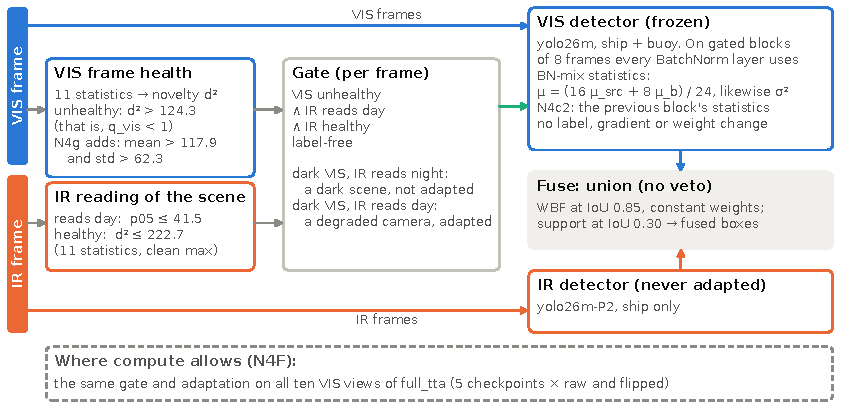
\includegraphics[width=1.0\linewidth]{figures/fig_n4_gate.pdf}
\caption{\textbf{IR-gated BatchNorm adaptation (\mbox{IG-BN}).} VIS: visible; IR: thermal infrared. Per frame and without labels, statistics of both cameras decide whether the frozen visible detector normalizes with BN-mix statistics re-estimated on a block of eight frames; the thermal detector is never adapted and the streams are fused by \textsc{union}. Each bound marked \emph{m} is the maximum of its statistic over clean development frames (day frames for the visible bounds), not a value tuned on detection scores.}
\label{fig:1}
\end{figure*}
\section{Related work}\label{sec:2}
\textbf{How test-time adaptation repairs a detector.} AdaBN \cite{li2017revisiting} replaces BatchNorm statistics with those of the test batch, and BN-mix \cite{schneider2020improving}, which \mbox{IG-BN} and the clock gate use unchanged, mixes them with the source statistics at a prior strength N. DUA \cite{mirza2022the} updates the statistics online with a decaying momentum and is evaluated on detection. TENT \cite{wang2021tent} and ActMAD \cite{mirza2023actmad} instead update parameters by gradient, minimizing entropy or aligning activation statistics at many layers; ActMAD applies to detectors. Because adapting where nothing shifted can hurt, some methods select which samples to adapt: SuMi \cite{guo2025smoothing} adapts only samples that pass feature-quartile and entropy tests. Others limit adaptation to some layers or weight source against test statistics per layer \cite{yang2022testtime,lim2023ttn,su2024unraveling,liao2026improving}; our shallow BN-mix (Section~\ref{sec:4.4}) combines both ideas.

\textbf{How multimodal methods decide what to adapt.} Several methods adapt only the shifted modality or reweight toward the reliable one. All of them decide from the model's own predictions or features and update parameters by gradient; they differ in the selection signal. TSA \cite{chen2025testtime} learns a router that chooses which modality to adapt, and reports negative transfer when an unshifted modality is adapted, the failure our gate guards against. AdaPGC \cite{xu2026multimodal} uses the divergence of each modality's prediction from the fused prediction, DASP \cite{he2026decoupling} the redundancy of the fused features, and CARAT \cite{mohapatra2026sourcelearned} each stream's own clean statistics; CARAT argues that cross-modal agreement misleads when sensors measure different physical processes. READ \cite{yang2024testtime}, ABPEM \cite{zhao2025attention} and MM-TTA \cite{shin2022mmtta} reweight the modalities inside the model, through attention or cross-modal pseudo-labels. These methods are evaluated on audio--video classification, sentiment, image--text classification, wearable time series and segmentation. The closest in sensors, Night-TTA \cite{liu2024testtime}, adapts night color--thermal segmentation by training BatchNorm affine parameters against an ensemble teacher, on every night frame, without deciding which frames to adapt.

\textbf{How visible--infrared detectors use illumination and uncertainty.} Illumination-aware fusion is established in multispectral pedestrian detection. IAF R-CNN \cite{li2019illuminationaware} weights its color and thermal sub-networks by an illumination estimate from the color image, and MBNet \cite{zhou2020improving} reweights and aligns modality features by illumination. ProbEn \cite{chen2022multimodal} fuses color and thermal detections by probabilistic ensembling. UA-CMDet \cite{sun2022dronebased} weights each object's training loss by cross-modal box overlap and RGB illumination, and at inference scales the RGB branch's scores by an illumination weight before non-maximum suppression. \citet{zhao2024uncertaintyaware} weight the visible and infrared branch losses by a label uncertainty estimated during training. All of these use illumination or uncertainty to set fusion weights, not to adapt a detector. Gaussian YOLOv3 \cite{choi2019gaussian} attaches per-coordinate variance to a single-stage detector; we use its head (Section~\ref{sec:6.1}).

\textbf{Maritime detection.} Maritime YOLO variants such as RDSC-YOLOv4 \cite{liu2021sea} and YOLOv7-Sea \cite{zhao2023yolov7sea} report accuracy without uncertainty or adaptation. Benchmarks for unmanned surface vehicles, MaSTr1325 \cite{bovcon2019the}, MODS \cite{bovcon2022mods} and LaRS \cite{zust2023lars}, are visible-only. The Pohang Canal dataset \cite{chung2023pohang} with PoLaRIS annotations \cite{choi2025polaris} provides paired visible--thermal maritime video with boxes on both streams; the Singapore Maritime Dataset \cite{prasad2017video} pairs visible with near-infrared video that need not show the same scene, and MassMIND \cite{nirgudkar2023massmind} is thermal only.

\textbf{The gap this paper addresses.} We found no test-time adaptation method for visible--infrared object detection among these papers. Ours differs from the multimodal methods in three ways. First, the decision \emph{whether} to adapt the visible detector comes from outside the model, from the thermal camera's own image or from a clock, rather than from agreement between model outputs; we compare these signals with shallow BN-mix, which weighs each block by its own statistics and needs neither. Second, no gradient is computed and no weight changes. Third, every variant was registered before it was scored. Selective adaptation of the corrupted modality is not our contribution, and neither is illumination-aware gating by itself, which IAF R-CNN and UA-CMDet apply to fusion weights.

\section{Setting}\label{sec:3}
\subsection{Data}\label{sec:3.1}
The Pohang Canal dataset \cite{chung2023pohang} records a 7.5 km route through a canal, a port and near-coastal water, not open sea, with a visible camera at 2048$\times$1080 and a thermal camera at 640$\times$512, both at 10 Hz. PoLaRIS \cite{choi2025polaris} supplies ship and buoy boxes on both streams. There are five runs: pohang00 (day), pohang01 (night), and pohang02 to pohang04 (day). The labeled streams hold 158,319 images, 1,183,736 boxes and 28,388 paired visible--infrared frames. The two cameras are not co-registered: frames are paired by nearest timestamp, and the measured residual misalignment is a median of 3--6 px per run. Visible frames are letterboxed to 640$\times$640; thermal frames are delivered as 8-bit images by per-frame min--max normalization, and the 14-bit radiometric values are not recoverable. Splits are interleaved contiguous blocks with guard bands, identical across modalities, and the night labels are the corrected set from a pre-registered restoration of boxes deleted from dark frames (Section~\ref{sec:6.2}).

\subsection{Detectors and fusion}\label{sec:3.2}
Both streams use YOLO26-m \cite{jocher2026ultralytics}: the visible detector with two classes, the thermal detector with a single ship class and an extra stride-4 (P2) detection level, because it cannot see buoys. The backbone was chosen on a 93-run benchmark (Section~\ref{sec:3.5}). We use five independently trained system pairs (visible seed k with thermal seed k), trained on the corrected labels with the held-out run removed from every list, and report the mean over the five.

The baseline fusion is \textsc{union}. Both streams pass to the Weighted Boxes Fusion (WBF) of \citet{solovyev2021weighted} at an intersection over union (IoU) of 0.85 with constant stream weights, and a box whose other-stream partner overlaps it at IoU 0.30 has its score multiplied by 1.5. At this threshold only 0.05 percent of visible boxes find a thermal partner, so the fusion is concatenation with a support bonus. The visible weight, 0.9926, is the constant that the designed uncertainty weighting produced on every frame (Section~\ref{sec:6.1}). The shipped system, \textsc{shipped}, is \textsc{union} plus a veto that drops the visible stream when the thermal camera indicates night and the visible frame reads dark or veiled. A registered study of replacements for that veto found that switching it off improves on it and that no gate we registered beats \textsc{union} (Section~\ref{sec:6.3}); \textsc{union} is therefore the baseline every adaptation is measured against. \textsc{full\_tta} (full test-time augmentation) is the strongest system that changes no detector: five checkpoints per stream, each run on the raw and the horizontally flipped frame, merged per stream by WBF at IoU 0.55, with non-local-means denoising of thermal frames that fail their health check, and no veto. It costs ten detector passes per stream per frame.

\subsection{Corruptions}\label{sec:3.3}
Adverse conditions are simulated on the content rows of each frame. Fog, low light and glare follow a camera-chain model in physical order: atmosphere, optics, sensor noise, exposure, the dataset's own infrared stretch and quantization. Fog is Koschmieder attenuation in linear radiance on per-frame metric depth \cite{sakaridis2018semantic} from Depth Anything V2 \cite{yang2024depth}. Low light is exposure scaling to the real night level, with the night noise measured on training frames. Glare is a source placed against the frame's computed horizon, with spread and exposure response fitted to the one real sun-entry event in training. Sensor noise, rain and motion blur are ImageNet-C-style severities \cite{hendrycks2019benchmarking} with no physical anchor. An earlier off-the-shelf corruption set was found broken at the source (its fog was a fixed 21-px blur) and retired. Sun glint, spray and salt on the lens were not modeled.

\subsection{Evaluation and statistics}\label{sec:3.4}
\textbf{Terms.} A \emph{cell} is one combination of visible condition, thermal condition and, on development, day or night. A \emph{draw} is one random realization of a corruption. VIS and IR denote the visible and infrared (thermal) streams scored alone. \emph{The no-loss property} is fused $\geq$ max(VIS, IR): the fused output scores at least as well as the better single stream.

\textbf{Development.} 2,232 paired validation frames, 1,200 by day (pohang00, 02, 03) and 1,032 by night (pohang01). The grid crosses five visible conditions (clean, fog at severities 1 and 2, low light, glare) with six thermal conditions (clean, fog at severities 1--3, noise at severities 2--3), by day and by night: 60 cells. It contains no visible noise, rain or blur. Corrupted cells average three draws per system; a cell's value is the mean over the five systems, with a 95 percent t-interval (df 4) on paired deltas.

\textbf{Held-out.} pohang04, an all-daylight run of 12,482 frame pairs, was never scored by any fusion system before its first pre-registered scoring, and neither the five system pairs nor their reference statistics were fitted on it. It has no thermal labels, so every held-out number is scored against the visible ground truth (156,652 boxes). Nine cells corrupt one stream at a time with four fresh draws each (visible fog, low light, sensor noise, rain and blur with clean thermal; clean visible with thermal fog, noise and blur; and clean/clean), and a tenth, visible glare, was added for the glare term. Held-out intervals are paired moving-block bootstraps over frames (block 20 frames, 1,000 replicates) around the five-system mean, because frames at 10 Hz are autocorrelated and a frame-level bootstrap halves the true width. They carry frame-sampling variance only, not variance over systems or draws, so they are not directly comparable with the development t-intervals.

\textbf{Metric and rule.} The metric is ship AP50--95 (local linear-interpolation AP), the only class both detectors emit. One rule decides every registered verdict, on development and held-out data alike: an arm passes (development) or replicates (held-out) if no cell is worse than its baseline by 0.0014 or more with the interval below zero, and at least one cell is better by 0.0060 or more with the interval above zero. The 0.0014 floor is the measured two-sigma noise of a paired delta; 0.0060 is the floor widened by the measured autocorrelation inflation. On held-out cells the development grid did not contain, the same rule is a first test, not a replication.

\textbf{Registration.} Each arm's prediction, cells, statistic and rule were written and committed before any of its numbers existed. No constant, threshold or calibration of any system was fitted on held-out labels, but two gate constants were chosen with the held-out run's label-free statistics (Section~\ref{sec:4.4}), and no untouched test set existed before it. The held-out run is scored only through registered tests, and each scoring is logged in an exposure ledger. It has been scored thirteen times: the original look of the shipped system, a re-score of its corrupted cells after the corruption model was replaced, and eleven later registrations: one of the gate-free systems (\textsc{union} and \textsc{full\_tta}), seven adaptation tests (Section~\ref{sec:5.2}), two scorings of the gate ablation (Section~\ref{sec:5.1}) and one of shallow BN-mix (Section~\ref{sec:5.1}). The evidence record names the variants by registration codes (\mbox{IG-BN} = N4, \mbox{IG-BN-causal} = N4c2, \mbox{IG-BN-stale} = N4c, \mbox{IG-BN+glare} = N4g, \mbox{IG-BN+ens} = N4F, \mbox{IG-BN+ens+glare} = N4Fg, \mbox{IG-BN+AE} = N4ae).

\subsection{Backbone benchmark}\label{sec:3.5}
Ninety-three runs, 31 YOLO variants from six families with three seeds each, were trained on the corrected labels and stopped after 20 epochs without a new best mAP50--95. Table~\ref{tab:1} lists the YOLO26 top tier and the best variant of each other family. The YOLO26 m, l and x variants differ by at most 0.0040, below the larger seed standard deviation of every pair, so the benchmark resolves a tier, not an order; the best variants of the other five families sit 0.010--0.025 below yolo26m. A selection rule fixed before the benchmark falls to throughput, where yolo26m runs at 57.0 frames per second against 30.7 for yolo26x. These are Ultralytics validation mAPs over ship and buoy on the full visible validation split, not the local ship AP of every other table, so no value here is comparable with them.

\begin{table*}[!t]
\centering
\small
\caption{Visible backbone benchmark, seed mean $\pm$ sd over three seeds}
\label{tab:1}
\begin{adjustbox}{max width=\linewidth}
\begin{tabular}{llrrr}
\toprule
Variant & Family & mAP50--95 & mAP50 & FPS \\
\midrule
yolo26x & YOLO26 & 0.2666 $\pm$ 0.0040 & 0.668 $\pm$ 0.033 & 30.7 \\
yolo26l & YOLO26 & 0.2664 $\pm$ 0.0070 & 0.677 $\pm$ 0.003 & 44.9 \\
yolo26m (selected) & YOLO26 & 0.2626 $\pm$ 0.0109 & 0.672 $\pm$ 0.026 & 57.0 \\
yolov10x & YOLOv10 & 0.2524 $\pm$ 0.0051 & 0.642 $\pm$ 0.010 & 34.9 \\
yolo12x & YOLO12 & 0.2523 $\pm$ 0.0091 & 0.641 $\pm$ 0.017 & 23.8 \\
yolov8l & YOLOv8 & 0.2470 $\pm$ 0.0033 & 0.634 $\pm$ 0.006 & 41.1 \\
yolo11x & YOLO11 & 0.2466 $\pm$ 0.0078 & 0.650 $\pm$ 0.022 & 29.0 \\
yolov9c & YOLOv9 & 0.2377 $\pm$ 0.0067 & 0.608 $\pm$ 0.018 & 43.6 \\
\bottomrule
\end{tabular}
\end{adjustbox}
\par\smallskip\raggedright\footnotesize Names as in Ultralytics; yolo26m is the YOLO26-m used throughout. The YOLO26 top tier and the best variant of each other family from the 93-run benchmark. Restored labels, stopped at patience 20, scored at the best epoch. FPS is one detector's \texttt{predict()} at fp32, batch 1, GPU clock pinned at 1,500 MHz.
\end{table*}
\section{Method}\label{sec:4}
\subsection{The ambiguity a single camera cannot resolve}\label{sec:4.1}
A degraded visible frame raises a question its own pixels cannot answer: is the scene dark, or is the camera failing? The visible health score is $q_{\mathrm{vis}}$ = min(1, 124.3/d$^{2}$), where d$^{2}$ is the Mahalanobis novelty of eleven frame statistics, fitted on clean day frames of the development runs, and 124.3 is its maximum over those frames; $q_{\mathrm{vis}}$ < 1 means d$^{2}$ > 124.3. The statistics are gradient Gini, mean gradient magnitude, the ratio of Laplacian variance to intensity variance, spectral slope, texture cover, the median ratio of local to global contrast, edge density, intensity standard deviation, the 5th-to-95th-percentile range, the log of the 95th-to-5th-percentile ratio and the fraction of dark pixels; the six heavy-tailed ones are log-compressed. It is a good detector of an unusual visible frame: it flags fogged, underexposed and noisy day frames. It is also, necessarily, a detector of night. On the development paired set it flags all 1,032 clean night frames as unhealthy and none of the 1,200 clean day frames. Night frames are in the visible detector's training distribution, and adapting them hurt on development (Section~\ref{sec:5.1}). Fig.~\ref{fig:10} shows the case. The thermal image's 5th-percentile intensity separates the two cases on development: clean day frames lie between 2 and 34 and clean night frames between 49 and 113 on its 8-bit scale. Because each thermal frame is stretched to its own minimum and maximum, this is a statistic of the stretched image, not of scene temperature; we have not established how much of the separation comes from the stretch.

\begin{figure*}[!t]
\centering
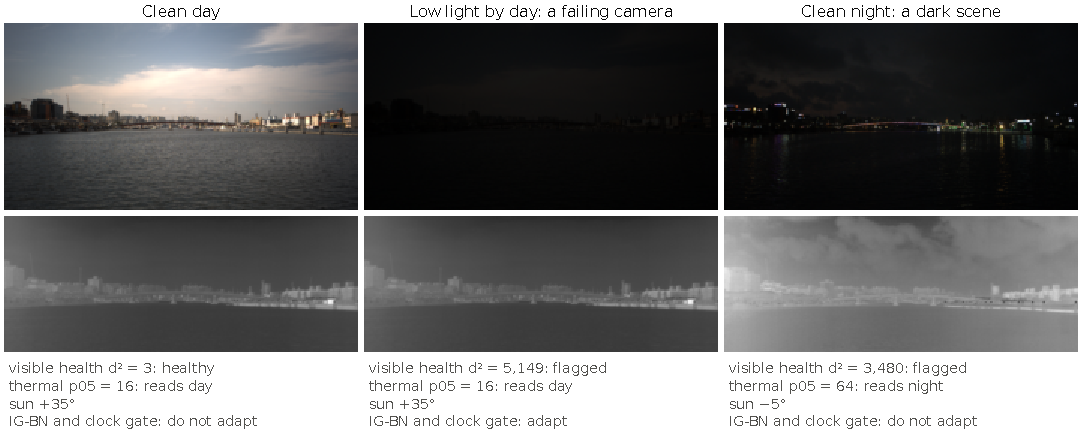
\includegraphics[width=1.0\linewidth]{figures/fig_ambiguity.pdf}
\caption{\textbf{The question every gate answers.} A pohang00 development frame, clean and under the registered low-light corruption, and a clean pohang01 night frame, each above its thermal partner. The visible health score flags both dark frames; the thermal 5th percentile and the sun tell the failing camera from the dark scene. In each run, the paired development frame with the most ground-truth ships; readings from the stored frame statistics of draw 942. Visible frames are shown without their letterbox pad and thermal frames as a centre band, for display only.}
\label{fig:10}
\end{figure*}
\subsection{The thermal gate (\mbox{IG-BN})}\label{sec:4.2}
The gate adapts a frame when the visible image looks wrong and the thermal camera reports daytime and is itself working. Per frame and without labels, it activates when three conditions hold:
\begin{itemize}
\item the visible frame is flagged as unhealthy: $q_{\mathrm{vis}}$ < 1;
\item the thermal frame reads daylight: its 5th-percentile intensity $p_{05}^{\mathrm{IR}}$ $\leq$ 41.5, the midpoint of the empty margin between clean day and clean night on development;
\item the thermal frame is itself healthy: the Mahalanobis novelty of its own eleven frame statistics is within 222.7, its maximum over clean development frames.
\end{itemize}

The third term exists because a degraded thermal stream can misread the scene: after the per-frame stretch, thermal fog and noise move a frame's 5th percentile across the day--night threshold, and without the health term the gate leaks onto up to 2.2 percent of night frames under thermal fog. With it, the gate activates on no night frame under any thermal condition on development. The threshold 41.5 was fitted on the same development frames on which this separation is shown.

\subsection{The adaptation}\label{sec:4.3}
Frames are taken in non-overlapping blocks of eight consecutive frames. Where the gate activates, every BatchNorm layer of the visible detector normalizes with the BN-mix statistics of \citet{schneider2020improving}:
\begin{equation*}\mu = \frac{N\mu_{\mathrm{src}} + n\mu_b}{N+n},\qquad \sigma^2 = \frac{N\sigma^2_{\mathrm{src}} + n\sigma^2_b}{N+n},\end{equation*}
with $N\,{=}\,16$, $n\,{=}\,8$, and $\mu_b$, $\sigma^2_b$ the block's statistics over its frames and spatial positions, computed layer by layer as the block passes through the network. Frames the gate does not pass keep the detector's plain output. No gradient is computed, no weight changes, no label is read, and the thermal detector is never adapted; the two streams are then fused by \textsc{union}.

\subsection{Variants}\label{sec:4.4}
Table~\ref{tab:22} lists the baselines, \mbox{IG-BN}'s variants and the other two answers, the clock gate and shallow BN-mix. \mbox{IG-BN} normalizes a block with its own statistics, which include up to seven later frames (0.7 s at 10 Hz); \mbox{IG-BN-causal} avoids this and is the version for a live stream. A first causal form, \mbox{IG-BN-stale}, reused the statistics of the previous block's adapted pass and failed by construction (Section~\ref{sec:5.1}). \mbox{IG-BN}'s gate almost never activates under glare, because a glared frame is bright and textured and does not look novel to $q_{\mathrm{vis}}$; the glare term covers that case. The clock gate keeps \mbox{IG-BN}'s visible term and replaces both thermal terms with the sun: it activates when $q_{\mathrm{vis}}$ < 1 and the solar elevation is above 0$^{\circ}$, computed from the frame's capture time and the nearest GPS fix. Shallow BN-mix drops the gate altogether. On every block it adapts only the first 31 of the detector's 130 BatchNorm layers, with the BN-mix weight $n/(N+n)\cdot\max(0,\,1 - D_0/D)$, where $D$ is the block's divergence from the training statistics at that layer (mean symmetric Kullback--Leibler divergence over channels) and $D_0$ its median over 240 clean training blocks. A block that looks like training data is left unchanged, by day or night. The layer count and the median were chosen on one development draw before registration.

\begin{table}[htbp]
\centering
\footnotesize
\caption{Systems and variants}
\label{tab:22}
\begin{tabularx}{\linewidth}{l>{\raggedright\arraybackslash}X}
\toprule
Name & What it is \\
\midrule
\textsc{union} & Baseline: both streams' boxes fused by WBF; no veto, no adaptation (Section~\ref{sec:3.2}) \\
\textsc{full\_tta} & Ensemble baseline: ten passes per stream (5 checkpoints $\times$ raw and flipped frame), no adaptation \\
\textsc{shipped} & Earlier system: \textsc{union} plus a night veto on the visible stream (Section~\ref{sec:6.2}) \\
\mbox{IG-BN} & \textsc{union} with the visible detector adapted on gated blocks (Sections~\ref{sec:4.2} and~\ref{sec:4.3}) \\
\mbox{IG-BN-causal} & Block b uses the statistics \mbox{IG-BN} measures on block b $-$ 1: no future frames, one extra pass per block \\
\mbox{IG-BN-stale} & First causal form: block b reused block b $-$ 1's adapted-pass statistics; dropped \\
\mbox{IG-BN+glare} & Gate also opens when visible mean > 117.9 and std > 62.3 (thermal terms unchanged) \\
\mbox{IG-BN+ens} & \mbox{IG-BN}'s gate and adaptation on all ten visible views of \textsc{full\_tta} \\
\mbox{IG-BN+ens+glare} & \mbox{IG-BN+ens} with \mbox{IG-BN+glare}'s gate \\
\mbox{IG-BN+AE} & Dark gated frames (mean linear luminance < 0.18) take an auto-exposed frame's detections \\
Clock gate & \mbox{IG-BN}'s visible term, with solar elevation > 0$^{\circ}$ in place of both thermal terms \\
Shallow BN-mix & No gate: BN-mix on the first 31 BatchNorm layers, weighted by the block's divergence from training statistics \\
\bottomrule
\end{tabularx}
\par\smallskip\raggedright\footnotesize The glare bounds are maxima over clean development day frames. AE: auto-exposure; ens: ensemble.
\end{table}
\textbf{Where the constants come from.} $N\,{=}\,16$ and the gate's terms were chosen on a preliminary screening draw before any development verdict; $N\,{=}\,64$ halved both the gains and the losses. The visible health bound, the thermal day threshold and the thermal health bound are the frozen constants of the shipped system, fitted on clean development frames. Two choices used the held-out run's label-free frame statistics before any of its scores existed. The thermal health term was switched from the shipped system's tighter bound, the 99th percentile of the same novelty over clean development frames, to its maximum (222.7) after the 99th-percentile bound was seen to pass only 9.5 percent of clean held-out thermal frames (the maximum passes 86.7 percent). The glare thresholds were checked to activate on 0.10 percent of clean held-out frames, after brightness percentiles that separate development glare perfectly were seen to activate on 55 percent of them. No constant was fitted on held-out labels.

\section{Results}\label{sec:5}
\subsection{Development}\label{sec:5.1}
\textbf{Ungated adaptation hurts on development.} In the pre-registered gate ablation below, BN-mix with $N\,{=}\,16$ on every frame gained on fogged and low-light day frames but changed ship AP by $-$0.0101 [$-$0.0147, $-$0.0055] on clean day frames, by $-$0.0195 [$-$0.0288, $-$0.0101] on clean night frames and by as much as $-$0.0233 on low-light night frames. A preliminary screen on one draw, not registered, had shown the same pattern. On unseen night frames it did not hold on average (Section~\ref{sec:5.3}). The gate is designed to keep the corrupted-frame gains and avoid the clean- and night-frame losses.

\textbf{IG-BN passes development} (Table~\ref{tab:2}). No cell of the 60 is worse than \textsc{union}; the worst $\Delta$ is $-$0.00001. Five are better beyond 0.0060 with intervals above zero: low light by day +0.0706 [+0.0593, +0.0818], low light with thermal fog at severity 1 +0.0357, visible fog at severity 1 +0.0094, visible fog at severity 2 +0.0091 and low light with thermal fog at severity 2 +0.0069. The gate activates on 16 cells, all by day: on 100 percent of low-light day frames and 99.6 percent of fogged day frames with clean thermal, and on no night frame under any thermal condition, so \mbox{IG-BN} equals \textsc{union} on every night cell. As thermal fog thickens the gate activates less, because the thermal stream no longer confirms daylight: on low-light day frames it activates on 42.5, 14.9 and 4.5 percent at thermal fog severities 1--3, and on none under thermal noise. Where fog degrades both bands, as real fog does, the gate therefore adapts few frames.

\begin{table*}[!t]
\centering
\footnotesize
\caption{Registered variants on development: 60 cells, five systems, ship AP, paired against the baseline named}
\label{tab:2}
\setlength{\tabcolsep}{3pt}
\begin{tabularx}{\linewidth}{lllrr>{\raggedright\arraybackslash}Xl}
\toprule
Variant & Change & Baseline & Better & Worse & Largest change [95\% CI] & Verdict \\
\midrule
\mbox{IG-BN} & gate + BN-mix & \textsc{union} & 5 & 0 & low light, day: +0.0706 [+0.0593, +0.0818] & PASS \\
\mbox{IG-BN+glare} & + glare term & \textsc{union} & 2 & 0 & glare, day: +0.0240 [+0.0178, +0.0302] & PASS \\
\mbox{IG-BN-stale} & stale statistics & \textsc{union} & 0 & 10 & low light, day: $-$0.1637 & FAIL \\
\mbox{IG-BN-causal} & previous block & \textsc{union} & 4 & 0 & low light, day: +0.0668 [+0.0559, +0.0777] & PASS \\
\mbox{IG-BN+AE} & + auto-exposure & \textsc{union} & 5 & 0 & low light, day: +0.0871 [+0.0734, +0.1008] & PASS \\
\mbox{IG-BN+ens} & in \textsc{full\_tta} & \textsc{full\_tta} & 5 & 0 & low light, day: +0.0696 [+0.0620, +0.0757] & PASS \\
\mbox{IG-BN+ens+glare} & + glare term & \textsc{full\_tta} & 2 & 0 & glare, day: +0.0179 [+0.0141, +0.0207] & PASS \\
\bottomrule
\end{tabularx}
\par\smallskip\raggedright\footnotesize Better and worse count cells beyond the rule's floors (Section~\ref{sec:3.4}); \mbox{IG-BN+ens} and \mbox{IG-BN+ens+glare} were scored on a second set of draws, with moving-block intervals because their arms are five-system ensembles.
\end{table*}
\textbf{The variants.} \mbox{IG-BN+glare} gains +0.0240 under glare by day and +0.0130 with the thermal stream in light fog; its worst cell is $-$0.0008. \mbox{IG-BN-stale} collapses from the first block that uses stale statistics, because they were measured under that block's own stale normalization rather than \mbox{IG-BN}'s: mean maximum confidence falls to 0.21 against \mbox{IG-BN}'s 0.75, and it was not taken further. \mbox{IG-BN-causal} passes; against \mbox{IG-BN} the price of causality is $-$0.0038 [$-$0.0045, $-$0.0031] on low-light day and within $\pm$0.0003 on fog. \mbox{IG-BN+AE} gains +0.0165 [+0.0053, +0.0278] over \mbox{IG-BN} on low light by day; darkness splits the conditions exactly, since every gated low-light frame is dark and no gated fog frame is, so on fog \mbox{IG-BN+AE} is \mbox{IG-BN}. Inside the ensemble, \mbox{IG-BN+ens}'s gain survives almost undiminished (+0.0696 on low-light day, on its own draws), and so does the glare gain (\mbox{IG-BN+ens+glare}, +0.0179 on glare by day). \mbox{IG-BN+ens+glare}'s rule had no gain requirement: no cell worse than \textsc{full\_tta}, and none below \mbox{IG-BN+ens} by 0.0014 where the glare term adds frames. The held-out build runs in half precision with fused batch statistics; a development check put its effect at no more than 0.0003.

\textbf{Which part of the gate does the work.} A pre-registered ablation scored the same adaptation under nine other gates. On development every prediction held: without a day--night term adaptation loses at night (to $-$0.0233), as does the feature-distribution gap of \citet{yoo2024what}, which activates on 90--100 percent of night frames. The day--night term need not come from the thermal camera: the visible term with solar elevation (the clock gate) is better than \textsc{union} on 17 cells and worse on none, and against \mbox{IG-BN} it is worse on no cell and better on 13 of the 15 fogged or low-light day cells with a corrupted thermal stream (+0.0709 [+0.0592, +0.0825] in low light under thermal noise). On the held-out daylight run, adapting every frame beats \mbox{IG-BN} on eight of nine cells (+0.0202 to +0.0216 on clean-visible cells), against the registered prediction. The sun is up on every held-out frame, so the held-out run cannot test the clock's day--night decision: there the clock gate is the visible term alone, which equals \mbox{IG-BN} on eight cells and beats it under visible noise (+0.0090).

\textbf{Adapting without any gate.} Shallow BN-mix (Section~\ref{sec:4.4}) needs neither a thermal camera nor a clock. It was registered on development draws 942--944 after a screen on draw 941. No cell is worse than \textsc{union} and 24 are better; against \mbox{IG-BN} it is better on 22 cells and worse on 2. Shallow BN-mix wins where \mbox{IG-BN}'s gate stays off: in mild visible fog with a degraded thermal stream (+0.0174 to +0.0212, against at most +0.0006 for \mbox{IG-BN}) and in low light by day under thermal fog or noise (+0.0558 to +0.0590, against at most +0.0069), because it does not depend on the thermal stream. It loses where \mbox{IG-BN} adapts every frame: low light by day ($-$0.0126 against \mbox{IG-BN}) and fog by day ($-$0.0033). Clean day frames move by at most 0.0002. Night is its weak side: clean and low-light night cells lie between $-$0.0046 and $-$0.0021, every interval crossing zero, within the registered $\pm$0.005 range and short of the worse-cell rule; on unseen night frames it moves by +0.0006 (Section~\ref{sec:5.3}). On the held-out run (a thirteenth registered scoring), it replicates (3 cells better, none worse): noise +0.1789, fog +0.0377 and low light +0.0088 over \textsc{union}. It is below \mbox{IG-BN} in low light ($-$0.0099) and, as registered, does not take the ungated arm's gain on clean held-out frames ($-$0.0003 against \textsc{union}; below ungated BN-mix on all nine cells).

\subsection{Held-out run}\label{sec:5.2}
Each variant that passed development was registered for the held-out run before any of its held-out numbers existed. None is worse than its baseline on any held-out cell (Table~\ref{tab:3}). Fog, low light and glare repeat development conditions and are replications; sensor noise, rain and blur are first tests.

\begin{table*}[!t]
\centering
\footnotesize
\caption{The held-out run (pohang04), one corrupted stream per cell, thermal stream clean in every corrupted row: ship AP against the visible ground truth}
\label{tab:3}
\setlength{\tabcolsep}{3pt}
\begin{tabularx}{\linewidth}{lrr>{\raggedright\arraybackslash}X>{\raggedright\arraybackslash}Xr>{\raggedright\arraybackslash}X}
\toprule
VIS condition & Gate & \textsc{union} & \mbox{IG-BN} $-$ \textsc{union} & \mbox{IG-BN-causal} $-$ \textsc{union} & \textsc{full\_tta} & \mbox{IG-BN+ens} $-$ \textsc{full\_tta} \\
\midrule
noise s2 (first test) & 85.2\% & 0.0169 & \textbf{+0.1823} [+0.1733, +0.1916] & \textbf{+0.1820 [+0.1730, +0.1913]} & 0.0206 & \textbf{+0.2174} [+0.2079, +0.2265] \\
fog & 67.8\% & 0.0445 & \textbf{+0.0370} [+0.0328, +0.0408] & \textbf{+0.0363 [+0.0323, +0.0401]} & 0.0586 & \textbf{+0.0445} [+0.0401, +0.0488] \\
glare s2 (+glare) & 81.0\% & 0.1417 & \textbf{+0.0309} [+0.0290, +0.0327] & \textbf{+0.0306 [+0.0287, +0.0325]} & 0.1656 & \textbf{+0.0311} [+0.0286, +0.0332] \\
low light & 85.2\% & 0.2152 & \textbf{+0.0186} [+0.0154, +0.0219] & \textbf{+0.0180 [+0.0148, +0.0212]} & 0.2458 & \textbf{+0.0190} [+0.0152, +0.0232] \\
rain s2 (first test) & 18.6\% & 0.2209 & +0.0036 [+0.0025, +0.0048] & +0.0035 [+0.0023, +0.0047] & 0.2534 & +0.0033 [+0.0022, +0.0047] \\
blur s3 (first test) & 9.2\% & 0.0419 & +0.0001 [+0.0000, +0.0001] & +0.0001 [+0.0000, +0.0001] & 0.0530 & +0.0000 [+0.0000, +0.0001] \\
clean (4 cells) & 0.0\% & 0.2635--0.2682 & 0 & 0 & 0.2923--0.2936 & 0 \\
\bottomrule
\end{tabularx}
\par\smallskip\raggedright\footnotesize Mean over the five systems and the four draws; $\Delta$ is paired against the arm's own baseline with a moving-block 95 percent interval, and Gate is the share of frames the gate passes. On the glare row each \mbox{IG-BN} column holds the +glare variant (\mbox{IG-BN+glare}, \mbox{IG-BN-causal+glare}, \mbox{IG-BN+ens+glare}) and Gate is its gate; \mbox{IG-BN} alone activates on 1.9 percent of glare frames. Bold: $\Delta$ $\geq$ +0.0060 with the interval above zero; s2, s3: severity; 0: $\Delta$ below 0.00005 (the gate passes no frame on three clean cells and a rounded 0.0 percent on the fourth).
\end{table*}
\textbf{IG-BN.} No cell is worse than \textsc{union}, and three are better beyond 0.0060 with intervals above zero. Under visible sensor noise, re-estimating the normalization statistics takes the fused output from 0.0169 to 0.1992; the ten-pass \textsc{full\_tta} reaches only 0.0206 there. This is the established benefit of BN re-estimation under noise \cite{schneider2020improving}, and a first test, since development has no visible noise. Fog gains +0.0370 and low light +0.0186, both in the direction seen on development. On the four cells with a clean visible stream (thermal clean, blurred, noisy or fogged) the gate activates on at most a rounded 0.0 percent of frames, so \mbox{IG-BN} equals \textsc{union} there to four decimals. Because every held-out frame is daylight and every corrupted-visible cell has a clean thermal stream, these cells exercise the gate's visible term; its day--night term is tested only at night, on development and on the night test (Section~\ref{sec:5.3}).

\textbf{IG-BN-causal.} The causal version keeps \mbox{IG-BN}'s held-out gains, with no cell worse: against \mbox{IG-BN} it costs at most 0.0007 (fog) on the held-out run and 0.0038 on development low light. With the glare term (\mbox{IG-BN-causal+glare}) it replicates on glare, 0.0003 below \mbox{IG-BN+glare}.

\textbf{IG-BN+glare.} None of the nine registered cells corrupts the visible stream with glare, so its registration added a tenth. There \mbox{IG-BN+glare} gains +0.0309 [+0.0290, +0.0327] over \textsc{union} (0.1417 to 0.1726), where \mbox{IG-BN} alone gains nothing, as on development; in the three other cells where the glare term adds two or three gated frames per draw, \mbox{IG-BN+glare} equals \mbox{IG-BN} to the fourth decimal.

\textbf{IG-BN+ens.} Inside the ensemble, no cell is worse than \textsc{full\_tta}. The gain is larger than \mbox{IG-BN}'s alone under noise (+0.2174 against +0.1823; 0.0206 to 0.2380) and fog (+0.0445 against +0.0370; 0.0586 to 0.1031), and the same under low light (+0.0190 against +0.0186) and rain (+0.0033 against +0.0036). Under glare, \mbox{IG-BN}'s gate activates on 1.9 percent of frames and \mbox{IG-BN+ens} equals \textsc{full\_tta}, so glare was registered separately with the glare term (\mbox{IG-BN+ens+glare}, after a development pass). It replicates: +0.0311 [+0.0286, +0.0332] over \textsc{full\_tta} (0.1656 to 0.1967), +0.0240 above one-pass \mbox{IG-BN+glare}, with no other cell worse than \mbox{IG-BN+ens}. On five of the six held-out cells with a corrupted visible stream, \mbox{IG-BN+ens} (\mbox{IG-BN+ens+glare} on glare) is the highest-scoring system we measured; under blur it ties \textsc{full\_tta}.

\textbf{IG-BN+AE, with a cost development could not show.} Low light gains +0.0259 [+0.0231, +0.0285] over \textsc{union}, +0.0073 [+0.0046, +0.0099] over \mbox{IG-BN}, as on development. But the held-out rain darkens every gated rain frame below auto-exposure's threshold, so auto-exposure replaces adaptation there and \mbox{IG-BN+AE} on rain is 0.0036 below \mbox{IG-BN}. Development has no rain. We do not recommend \mbox{IG-BN+AE} for that reason.

Fig.~\ref{fig:9} shows one held-out frame under the three conditions.

\begin{figure*}[!t]
\centering
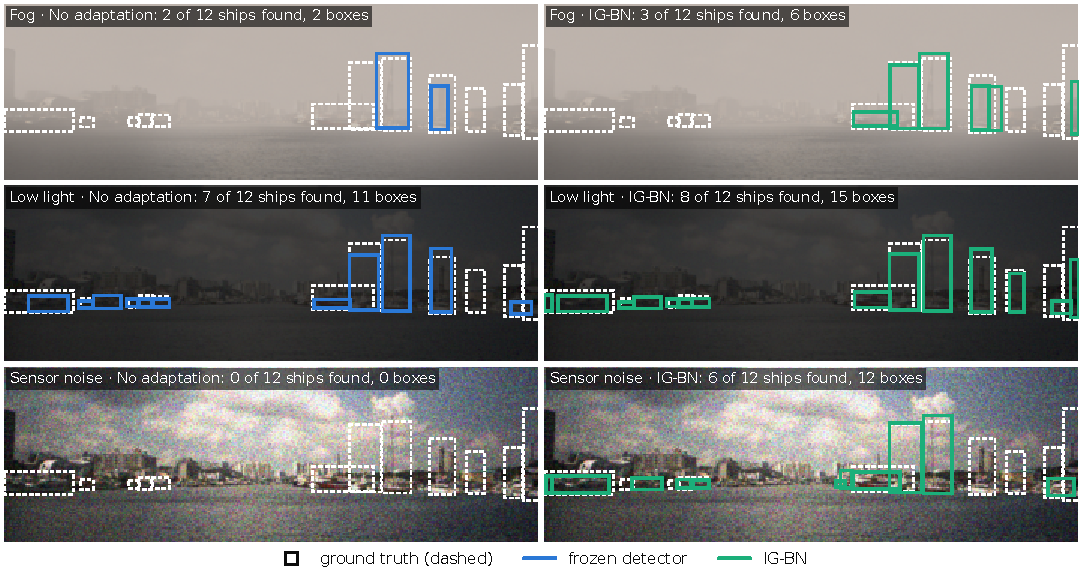
\includegraphics[width=1.0\linewidth]{figures/fig_tta_detections.pdf}
\caption{\textbf{IG-BN on one held-out frame, thermal stream clean.} pohang04 frame 9042, system seed 0, corruption draw 941. Left, the frozen visible detector, the stream \textsc{union} fuses; right, the same detector with \mbox{IG-BN}, whose gate activates on this frame under all three conditions. Ship boxes at confidence $\geq$ 0.25 over the dashed ground truth; \emph{found} counts ground-truth ships matched at IoU $\geq$ 0.5. Every box is read from the records the held-out scorings used (\mbox{IG-BN} in fp16); nothing was re-run. The frame was chosen on ground truth alone: of the 5,237 frames where the gate activates under all three conditions and at least three ships are labeled, the one with the largest median ship height times ship count (capped at six). Low light is brightened for display (gamma 0.45); the detector saw the stored frame. One frame shows the mechanism, not the size of the gain, which is in Table~\ref{tab:3}.}
\label{fig:9}
\end{figure*}
\subsection{Where \mbox{IG-BN}'s gate stays off, and a night test}\label{sec:5.3}
The gate activates on no frame of the clean held-out cell, on a rounded 0.0 percent of the other clean-visible held-out cells, and on no development night frame under any thermal condition, so on those frames every variant equals its baseline. That matters because the baseline is already strong there. At night, \textsc{union} keeps the visible stream that the shipped veto discards. On a night test registered on pohang01's test split, 1,109 frame pairs that no fusion system had scored, \textsc{union} beats \textsc{shipped} by +0.0273 [+0.0154, +0.0400] and holds the no-loss property at $-$0.0010 [$-$0.0049, +0.0031], while \textsc{shipped}, which vetoes the visible stream on 90.3 percent of those frames, fails it by 0.0283. The detectors trained on the same run's training split, so this tests the fusion rule, not the detectors, and night AP levels swing from 0.04 to 0.35 between the run's 52-second episodes; directions, not levels, transfer. \mbox{IG-BN}'s gate, measured without labels, activates on 1 of 17,744 pair-draws (one thermal-fog draw) against a registered prediction of none, so \mbox{IG-BN} equals \textsc{union} on this night test. The thermal terms alone would not keep the gate off: under thermal fog the thermal stream reads day on 37--42 percent of these night pairs, and the health term rejects all but the one. A solar gate activates on none (the sun is 6--10$^{\circ}$ below the horizon), the feature-gap gate of Section~\ref{sec:5.1} on 99.3 percent with the thresholds of \citet{yoo2024what} and on 66.5 percent with calibrated ones.

\textbf{Adapting on the night test.} A second registration on these pairs scored the two answers that adapt at night (\mbox{IG-BN} and the clock gate adapt none). Shallow BN-mix moves \textsc{union} by +0.0006 [$-$0.0020, +0.0031], as registered. Ungated BN-mix, predicted to be worse as on development night ($-$0.0195), is better: +0.0106 [+0.0043, +0.0163], from +0.0178 on one stretch and $-$0.0099 on the other. The evidence that adapting the whole network needs a day--night signal therefore rests on development.

\begin{figure*}[!t]
\centering
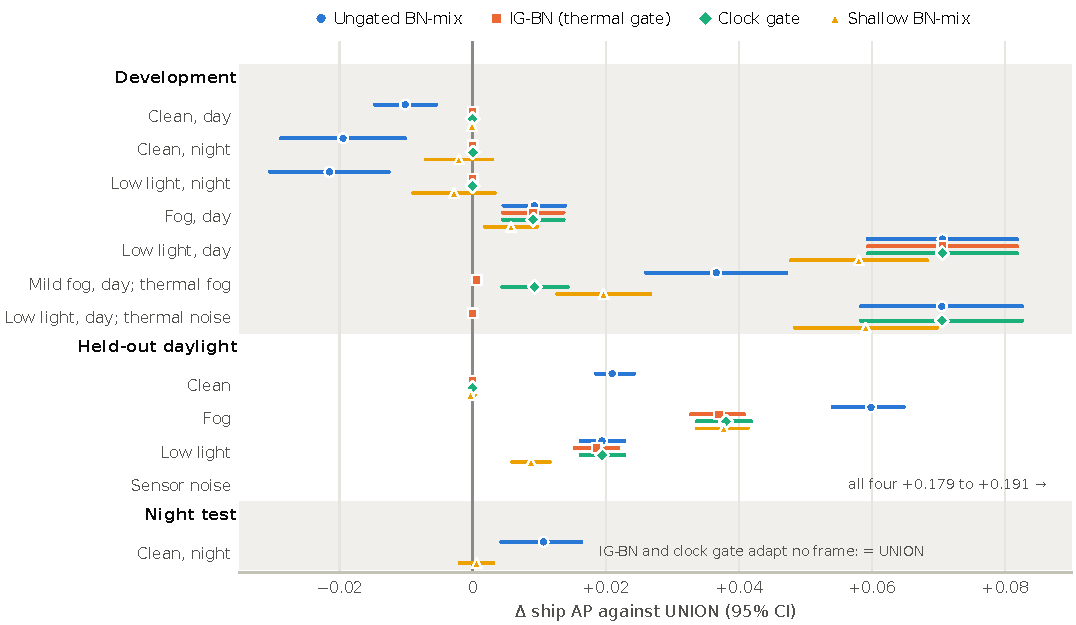
\includegraphics[width=1.0\linewidth]{figures/fig_three_answers.pdf}
\caption{\textbf{The three answers and ungated BN-mix on each kind of test.} $\Delta$ ship AP against \textsc{union} with 95\% intervals: development cells (five systems, draws 942--944, t-intervals), the held-out daylight run (pohang04, moving-block intervals) and the night test (pohang01 test split, moving-block intervals). \mbox{IG-BN} and the clock gate adapt no night-test frame and equal \textsc{union} there, so they are labelled rather than drawn. Under held-out sensor noise all four gain +0.179 to +0.191, beyond the axis.}
\label{fig:11}
\end{figure*}
\subsection{An observation, not a test: ranking the adapted streams}\label{sec:5.4}
\mbox{IG-BN} inherits a weakness of \textsc{union}. Where the visible stream is clean, the fused output falls below the visible stream alone, by 0.0085 to 0.0132 on the held-out run, because the thermal stream's boxes are interleaved with the visible stream's. A fixed ordering that ranks every visible box above every thermal box (\textsc{lex}) cannot fall below the visible stream: the scorer matches boxes greedily in score order, so a tail of boxes appended below every existing box cannot lower AP. The same ordering of \mbox{IG-BN}'s adapted streams scores above \mbox{IG-BN} in all nine held-out cells, by +0.0096 to +0.0134 where the visible stream is clean and +0.0008 to +0.0067 where it is corrupted, and it holds the no-loss property in every cell. No verdict was registered for it, and on development \textsc{lex} averaged 0.0037 below \textsc{union} over the 60 cells. The two data sets disagree, so we report it as a candidate for the next registration and keep \textsc{union}, as registered, with the adaptation chosen by Table~\ref{tab:23}. The visible detector with \mbox{IG-BN} and no thermal boxes at all was not scored as a system.

\section{What did not work on the same system}\label{sec:6}
Earlier registered attempts to use the second sensor shaped the designs of Section~\ref{sec:4}; we summarize them here.

\subsection{Predicted uncertainty is informative but does not improve the fusion}\label{sec:6.1}
Each detector carries a Gaussian variance head \cite{choi2019gaussian} trained with a beta-weighted negative log-likelihood \cite{seitzer2022on}, and the system was designed so that predicted $\sigma$ would weight the fusion. We pre-registered the comparison that answers whether it should: real $\sigma$ against the same $\sigma$ shuffled onto the wrong boxes, at least three of four conditions above 0.0060 with a block-bootstrap interval excluding zero. Used as a weight on box coordinates, $\sigma$ passes on none of four conditions (the fusion weight took one value on every frame, Section~\ref{sec:3.2}). Used to re-rank scores, real $\sigma$ beats shuffled $\sigma$ on three of four conditions, so it carries information about which boxes are right. But that information is within each detector: by day the gain is the visible detector re-ranking its own boxes, and adding the thermal stream moves it by $-$0.0040 to +0.0035 with no consistent sign. Against the system with no $\sigma$ at all, the re-ranked system scores lower on six of eight cells. A shuffled control establishes that a signal exists, not that using it helps. Learned jointly with confidence in a re-ranker of the visible boxes, $\sigma$ adds +0.0050 [+0.0038, +0.0064] on one checkpoint, and its pre-registered replication on the five retrained detectors failed: positive on all five, beyond the floor on two. The recorded runs had first scored a ship-and-buoy macro instead of the registered ship AP. Under physically modeled corruptions, re-ranking passes on only one or two of four conditions.

\subsection{A sensor veto is a claim about the detector}\label{sec:6.2}
The system that shipped dropped the visible stream when the thermal camera voted night and the visible frame read dark or veiled. Its night arm was written while the visible detector scored 0.0000 at night. That zero turned out to be a label artifact: a filter had deleted every box in dark night frames from the training labels, and a registered restore of the boxes took night visible mAP50--95 from 0.0000 to 0.2520. Retrained on the corrected labels, the visible detector sees at night, and the unchanged rule discards it: on clean night the fused output equals the thermal stream alone and falls 0.1847 [0.1655, 0.2039] below the visible stream. The images did not change; the detector did, and the rule's assumption about it no longer held. The rule gated on darkness, while what decides whether the visible stream should be dropped is its health, and with the retrained detector those variables no longer coincide. The thermal side shows the same failure: under a fogged or noisy thermal stream, the veto's fallback reads a dark low-light day as a fogged night and vetoes a working visible stream on up to 96 percent of day frames. \mbox{IG-BN}'s gate keeps the two apart: it reads day or night from the thermal stream and health from each stream.

\subsection{No learned gate beat removing the veto}\label{sec:6.3}
Seven learned or hand-written replacements for the veto were registered and scored on fresh corruption draws. None beat switching the veto off: \textsc{union} is better than \textsc{shipped} on 30 of 60 development cells and worse on none, and every gate was worse than \textsc{shipped} somewhere by day. Two mechanisms explain most of it. A model of box correctness fitted to a noisy matching target re-orders a detector's own boxes worse than its confidence does. And a frame-level gate pools frames whose scores live on different scales: switching to the visible stream alone on a random three quarters of frames, a choice that carries no information, scores 0.0085 below the interpolation between the two pure policies. The largest gain came from ensembling frozen checkpoints, not from fusion: it helps every arm it is put under, and \textsc{full\_tta} beats \textsc{shipped} on 57 of 60 development cells and on all nine held-out cells. The adaptation, the one change here that acts inside a detector, adds to the ensemble.

\section{Discussion}\label{sec:7}
\begin{table*}[!t]
\centering
\small
\caption{Which answer to use}
\label{tab:23}
\begin{tabularx}{\linewidth}{llrr>{\raggedright\arraybackslash}X}
\toprule
Signals & Use & Development & Held-out & Caveat \\
\midrule
Time and position & Clock gate & 17 / 0 & 3 / 0 & untested at dusk, dawn, overcast \\
Thermal camera only & \mbox{IG-BN} & 5 / 0 & 3 / 0 & adapts little when thermal degraded \\
Neither & Shallow BN-mix & 24 / 0 & 3 / 0 & dev night $-$0.0046 to $-$0.0021; night test +0.0006 \\
\bottomrule
\end{tabularx}
\par\smallskip\raggedright\footnotesize Cells better / worse than \textsc{union} (Section~\ref{sec:3.4}); held-out: pohang04, all daylight, where the clock gate is the visible term alone.
\end{table*}
\textbf{What the thermal camera contributes, and what is not yet shown.} As a second detector scored against the visible labels, the thermal stream adds little by day on this data: on the held-out run it scores 0.0156 against the visible stream's 0.2767, and fusing it lowers the output wherever the visible stream is clean (Section~\ref{sec:5.4}). That comparison is confounded: the held-out run has visible labels only, so a true thermal-only detection counts as a false positive, and against its own labels on development the thermal detector scores 0.141 ship AP by day, against the visible detector's 0.378 on the same frames. As a gate, the thermal camera separated a dark scene from a degraded camera on development, where an underexposed visible frame and a night frame look alike to every statistic of the visible frame we tried. The pre-registered ablation (Section~\ref{sec:5.1}) shows on development that the separation is needed and that the thermal camera is not needed to make it. The night test (Section~\ref{sec:5.3}) did not reproduce the ungated night loss on average. The thermal reading is needed only where a clock misjudges the light the camera sees: dusk, dawn, heavy overcast, bridges and covered berths. None occur in this data.

\textbf{What we recommend.} For a two-stream detector built from frozen detectors: fuse by \textsc{union}, without a night veto, and adapt the visible detector with BN-mix. Which frames to adapt depends on the signals available (Table~\ref{tab:23}, Fig.~\ref{fig:11}). Where time and position are known, decide day and night with the clock: on this data it served better than the thermal reading, which needs its own health check, since thermal fog makes it read day on up to 42 percent of night frames (Section~\ref{sec:5.3}). Where only the thermal camera can tell, use \mbox{IG-BN}, the most tested of the three and the only one tested in causal and ensemble forms; the other two were tested only on blocks that include later frames. Where neither is available, shallow BN-mix adapts without a day--night signal. It comes last despite winning the most development cells: it alone adapts at night, where its night changes are within noise, all negative on development ($-$0.0046 to $-$0.0021) and +0.0006 on unseen night frames, and it trails \mbox{IG-BN} in low light and fog by day. It and the clock gate were not compared directly. On whether to adapt every frame or only flagged ones, development and the held-out tests disagree, by day (Section~\ref{sec:5.1}) and on average at night (Section~\ref{sec:5.3}); the gated forms and shallow BN-mix are the conservative choices.

\textbf{A note on the protocol.} A measured paired noise floor, block-bootstrap intervals and magnitude floors moved 20 of 74 earlier findings of this project to indeterminate when applied retroactively, and a registration exposed a wrong metric in its own recorded runs (Section~\ref{sec:6.1}). \mbox{IG-BN}'s gains survive these corrections: its smallest headline gain, +0.0186, is nearly eight times the 0.0024 maximum of the ship-AP noise floor.

\section{Conclusion}\label{sec:8}
On our development set, test-time adaptation of a visible detector helped on degraded frames and hurt on clean and night frames, because a visible camera cannot tell a dark scene from a dark sensor. We compared three pre-registered answers. Gating BatchNorm re-estimation on a co-mounted thermal camera's reading of daylight and on both streams' health (\mbox{IG-BN}) kept the gains with no development or held-out cell worse. On one held-out daylight run it replicated under fog, low light and glare, and gained +0.18 ship AP under sensor noise in a first test. The clock gate did at least as well as \mbox{IG-BN} on development, though the all-daylight held-out run could not test its day--night decision. Adapting only the shallow layers, in proportion to each block's drift from the training statistics, needed no day--night signal and was worse than the baseline on no cell, with night changes within noise on development and on unseen night frames. Which to use depends on the signals a vessel has (Table~\ref{tab:23}). Whether any frame needs gating is open: adapting every frame did best on both held-out tests, on average. The same system's earlier attempts to use the second sensor, as an uncertainty-weighted voter and as a sensor veto, did not survive registration.

\textbf{Data and code availability.} The Pohang Canal images and PoLaRIS labels are public \cite{chung2023pohang,choi2025polaris}. The code, every pre-registration as a dated commit, the exposure ledger and the result record behind each table and figure are in the public repository github.com/Laksh-saroha/maritime-tta.

\FloatBarrier
\bibliographystyle{IEEEtranN}
\bibliography{references}

\end{document}
